\documentclass[a4paper,twoside,openright,makeidx,12pt]{book}
%\usepackage{draftcopy}
%$Id: macro.tex,v 1.10 2004/12/08 13:38:58 acary Exp $


%\usepackage{a4wide}
\textheight 25cm
\textwidth 16.5cm
\topmargin -1cm
%\evensidemargin 0cm
\oddsidemargin 0cm
\evensidemargin0cm
\usepackage{layout}


\usepackage{amsmath}
\usepackage{amssymb}
\usepackage{minitoc}
%\usepackage{glosstex}
\usepackage{colortbl}
\usepackage{hhline}
\usepackage{longtable}

%\usepackage{glosstex}
%\def\glossaryname{Glossary of Notation}
\def\listacronymname{Acronyms}

\usepackage[outerbars]{changebar}\setcounter{changebargrey}{20}
%\glxitemorderdefault{acr}{l}

%\usepackage{color}
\usepackage{graphicx,epsfig}
\graphicspath{{./Figures/}}
\usepackage[T1]{fontenc}
\usepackage{rotating}

%\usepackage{algorithmic}
%\usepackage{algorithm}
\usepackage{ntheorem}
\usepackage{natbib}


%\renewcommand{\baselinestretch}{2.0}
\setcounter{tocdepth}{2}     % Dans la table des matieres
\setcounter{secnumdepth}{3}  % Avec un numero.



\newtheorem{definition}{Definition}
\newtheorem{lemma}{Lemma}
\newtheorem{claim}{Claim}
\newtheorem{remark}{Remark}
\newtheorem{assumption}{Assumption}
\newtheorem{example}{Example}
\newtheorem{conjecture}{Conjecture}
\newtheorem{corollary}{Corollary}
\newtheorem{OP}{OP}
\newtheorem{problem}{Problem}
\newtheorem{theorem}{Theorem}


\newcommand{\CC}{\mbox{\rm $~\vrule height6.6pt width0.5pt depth0.25pt\!\!$C}}
\newcommand{\ZZ}{\mbox{\rm \lower0.3pt\hbox{$\angle\!\!\!$}Z}}
\newcommand{\RR}{\mbox{\rm $I\!\!R$}}
\newcommand{\HH}{\mbox{\rm $I\!\!H$}}
\newcommand{\NN}{\mbox{\rm $I\!\!N$}}

\newcommand{\Mnn}{\mathcal M^{n\times n}}
\newcommand{\Mnp}[2]{\ensuremath{\mathcal M^{#1\times #2}}}



\newcommand{\Frac}[2]{\displaystyle \frac{#1}{#2}}

\newcommand{\DP}[2]{\displaystyle \frac{\partial {#1}}{\partial {#2}}}

% c++ variables writting
\newcommand{\varcpp}[1]{\textit{#1}}
% itemize
\newcommand{\bei}{\begin{itemize}}
\newcommand{\ei}{\end{itemize}}

\newcommand{\ie}{i.e.}
\newcommand{\eg}{e.g.}
\newcommand{\cf}{c.f.}
\newcommand{\putidx}[1]{\index{#1}\textit{#1}}

\def\Er{{\rm I\! R}}
\def\En{{\rm I\! N}} 
\def\Ec{{\rm I\! C}}
 
\def\zc{\hat{z}}
\def\wc{\hat{w}}

\font\tete=cmr8 at 8 pt


% normal tangent
\def\n{{\hbox{\tiny{N}}}}
\def\t{{\hbox{\tiny{T}}}}
\def\nt{\hbox{\tiny{NT}}}
\def\nsf{\hbox{\tiny{\textsf N}}}
\def\tsf{\hbox{\tiny{\textsf T}}}
\def\sigman{\sigma_{\n}}
\def\sigmat{\sigma_{\t}}
\def\sigmant{\sigma_{\nt}}
\def\epsn{\epsilon_{\n}}
\def\epst{\epsilon_{\t}}
\def\epsnt{\epsilon_{\nt}}
\def\eps{\epsilon}
\def\veps{\varepsilon}
\def\sig{\sigma}
\def\Rn{R_{\n}}
\def\Rt{R_{\t}}
\def\cn{c_{\n}}
\def\Cn{C_{\n}}
\def\ct{c_{\t}}
\def\Ct{C_{\t}}
\def\un{u_{\n}}
\def\ut{\buu_{\t}}
\def\uut{u_{\t}}
\def\unc{u_{\n}^c}
\def\utc{\buu_{\t}^c}
\def\vn{v_{\n}}
\def\vt{v_{\t}}
\def\rr{\hbox{\tiny{\textsf R}}}
\def\irr{\hbox{\tiny{\textsf{IR}}}}
\def\rn{r_{\n}}
\def\rt{\brr_{\t}}
\def\rnc{r_{\n}^c}
\def\rtc{\brr_{\t}^c}
\def\trn{\Tilde{r}_{\n}}
\def\trt{\Tilde{\brr}_{\t}}
\def\tr{\Tilde{\brr}}
\def\tv{\Tilde{\bvv}}
\def\vn{v_{\n}}
\def\vt{\bvv_{\t}}
\def\adh{\mathsf{adh}}
\def\adj{\hbox{\tiny{\textsf{adj}}}}
\def\adjc{\hbox{\tiny{\textsf{adjC}}}}
\def\adja{\hbox{\tiny{\textsf{adjA}}}}
\def\cc{\hbox{\tiny{\textsf C}}}
\def\ca{\hbox{\tiny{\textsf A}}}

\DeclareMathOperator{\proj}{proj}
\DeclareMathOperator{\expm}{expm}
\DeclareMathOperator{\dexp}{dexp}
\DeclareMathOperator{\dlexp}{d^l exp}
\DeclareMathOperator{\drexp}{d^r exp}
\DeclareMathOperator{\dexpm}{dexpm}
\DeclareMathOperator{\expq}{expq}
\DeclareMathOperator{\dexpq}{dexpq}
\DeclareMathOperator{\Ad}{Ad}
\DeclareMathOperator{\ad}{ad}
\DeclareMathOperator{\dd}{d}



%%  Les ensembles de nombres  C. Fiorio (fiorioÊatÊmath.tu-berlin.de) 
%
\def\nbR{\ensuremath{\mathrm{I\!R}}} % IR
\def\nbN{\ensuremath{\mathrm{I\!N}}} % IN
\def\nbF{\ensuremath{\mathrm{I\!F}}} % IF
\def\nbH{\ensuremath{\mathrm{I\!H}}} % IH
\def\nbK{\ensuremath{\mathrm{I\!K}}} % IK
\def\nbL{\ensuremath{\mathrm{I\!L}}} % IL
\def\nbM{\ensuremath{\mathrm{I\!M}}} % IM
\def\nbP{\ensuremath{\mathrm{I\!P}}} % IP

%----------------------------------------------------------------------
%                  Modification des subsubsections
%----------------------------------------------------------------------
\makeatletter
\renewcommand\thesubsubsection{\thesubsection.\@alph\c@subsubsection}
\makeatother

%----------------------------------------------------------------------
%             Redaction note environnement
%----------------------------------------------------------------------
\makeatletter
\theoremheaderfont{\scshape}
\theoremstyle{marginbreak}
\theorembodyfont{\upshape}
%\newtheorem{rque}{\bf Remarque}[chapter]
%\newtheorem{rque1}{\bf \fsc{Remarque}}[chapter] !!! \fsc est une commande french
\newtheorem{ndr1}{\textbf{\textsc{Redaction note}}}[section]

\newenvironment{ndr}%
{%
\tt
%\centerline{---oOo---}
\noindent\begin{ndr1}%
}%
{%
\begin{flushright}%
%\vspace{-1.5em}\ding{111}
\end{flushright}%
\end{ndr1}%
%\centerline{---oOo---}
}

\makeatother

%----------------------------------------------------------------------
%             Redaction note environnement V.ACARY
%----------------------------------------------------------------------
\makeatletter
\theoremheaderfont{\scshape}
\theoremstyle{marginbreak}
\theorembodyfont{\upshape}
%\newtheorem{rque}{\bf Remarque}[chapter]
%\newtheorem{rque1}{\bf \fsc{Remarque}}[chapter] !!! \fsc est une commande french
\newtheorem{ndr1va}{\textbf{\textsc{Redaction note V. ACARY}}}[section]

\newenvironment{ndrva}%
{%
\tt
%\centerline{---oOo---}
\noindent\begin{ndr1va}%
}%
{%
\begin{flushright}%
%\vspace{-1.5em}\ding{111}
\end{flushright}%
\end{ndr1va}%
%\centerline{---oOo---}
}

\makeatother
%----------------------------------------------------------------------
%             Redaction note environnement V.ACARY
%----------------------------------------------------------------------
\makeatletter
\theoremheaderfont{\scshape}
\theoremstyle{marginbreak}
\theorembodyfont{\upshape}
%\newtheorem{rque}{\bf Remarque}[chapter]
%\newtheorem{rque1}{\bf \fsc{Remarque}}[chapter] !!! \fsc est une commande french
\newtheorem{ndr1fp}{\textbf{\textsc{Redaction note F. PERIGNON}}}[section]

\newenvironment{ndrfp}%
{%
\tt
%\centerline{---oOo---}
\noindent\begin{ndr1fp}%
}%
{%
\begin{flushright}%
%\vspace{-1.5em}\ding{111}
\end{flushright}%
\end{ndr1fp}%
%\centerline{---oOo---}
}

\makeatother
%----------------------------------------------------------------------
%                  Chapter head enviroment
%----------------------------------------------------------------------
\newenvironment{chapter_head}
{%
\begin{center}%
-------------------- oOo --------------------\\%
\ \\%
\begin{minipage}[]{14cm}%
\noindent\normalsize\advance\baselineskip-1pt %
}%
{%
\par\end{minipage}%
\ \\%
\ \\%
-------------------- oOo --------------------
\end{center}%
\vspace*{\stretch{1}}%
\clearpage%
\thispagestyle{empty}%
\vspace*{\stretch{1}}%
\minitoc%
\vspace*{\stretch{2}}%
\clearpage%
}


\newcommand{\contract}{{\,:\,}}

%%% Local Variables: 
%%% mode: latex
%%% TeX-master: "report"
%%% End: 


\includeonly{}
\usepackage{fancyheadings} 

% package pour les images des use cases
%\usepackage[dvips]{graphicx}

\pagestyle{fancy} 
\renewcommand{\chaptermark}[1]% 
{\markboth{{Chap-- \thechapter.\ #1}}{}} 
\renewcommand{\sectionmark}[1]% 
{\markright{{\thesection.\ #1}}} 
\setlength{\headrulewidth}{0.5pt} 
\setlength{\footrulewidth}{0.5pt} 
\newcommand{\helv}{% 
\fontfamily{phv}\fontseries{b}\fontsize{9}{11}\selectfont} 
\lhead[\helv \thepage]{\helv \rightmark} 
\rhead[\helv \leftmark]{\helv \thepage} 
\cfoot{Architectural Design Document -- \today}

\makeindex

\begin{document}
\pagestyle{empty}
\renewcommand{\arraystretch}{1.8}

%%%%%%%%%%%%%%%%%%%%%%%%%%%%%%%%%%%%%%%%%%%%%%%%%%%%%%%%%%%%%%%%%%%%%%%%%%%%%%%%

\thispagestyle{empty}

\begin{center}
\includegraphics[height=23mm, width=77mm]{figure/siconos.eps}\\
\textsf{Siconos Project}\\[6cm]
\end{center}

\begin{center}
\huge
\textsf{\textbf{\textit{Architectural Design Document}}}\\[2.5cm]
\end{center}

\large
\begin{center}
\textsf{\textbf{Version :} 1.0}\\
\textsf{\textbf{Status :}  Validated}\\
\textsf{\textbf{Date : } March 29, 2004}\\
\textsf{\textbf{Document Code :} \acs{add}}\\[5cm]

\end{center}

\normalsize

\begin{flushright}

\includegraphics[scale=0.3]{figure/Logo-INRIA.eps}
\end{flushright}

\clearpage




%\maketitle

%-----------------------------------------------------------------------------%

\normalsize

\begin{center}
  \textsf{\Large Identification}
\end{center}

\noindent\begin{tabular}{|p{0.3\textwidth}|p{0.7\textwidth}|}
\hline
Document Title : & \textsf{Architectural Design Document} \\
Document Code :  & \textsf{\acs{add}} \\
\hline
\end{tabular}
\textsf{ }\\


\begin{center}
  \textsf{\Large About the document and its author(s)}
\end{center}

\noindent\begin{tabular}{|p{0.3\textwidth}|p{0.7\textwidth}|}
\hline
Nature :& \textsf{This document defines the global architecture of the
platform}\\
Language :& \textsf{English}\\
Author(s) :& \textsf{Jean-Michel Barbier - Alexandre Ravoux}\\
Possible remarks :& \textsf{This document describe the whole platform}\\
References : &\textsf{\acs{srd}, \acs{esd}, \acs{op}, \acs{pti}}\\
\hline
\end{tabular}

\textsf{ }\\

%\newpage




% cartridge current version
\renewcommand{\arraystretch}{1.2}
\begin{center}
  \textsf{\Large Current Version}
\end{center}
\begin{tabular}{|p{0.3\textwidth}|p{0.7\textwidth}|}
\hline
Date : &\textsf{MArch 25, 2004}\\
Current version number : &\textsf{1.0}\\ 
Status :&$\bigcirc$ in progress \\
& $\bigotimes$ validated\\
\textit{ }& \hspace{0.5cm} Approved by : J�r�mie Blanc-Tranchant\\
\hline
\end{tabular}


\textsf{ }\\
\begin{center}
\textbf{Copyright Notice \copyright}\\
This document may not be reproduced (even partially) or communicated to third parties without the written authorisation of INRIA.
\end{center}
\renewcommand{\arraystretch}{1.8}


% log of changes  
\pagebreak
\begin{center}
  \textsf{\Large About the document developing process}
\end{center}
\begin{tabular}{|p{0.3\textwidth}|p{0.7\textwidth}|}
\hline
Date of first issue : &\textsf{March 25, 2004}\\
Current version number : &\textsf{1.0}\\ 
Validated by :& \textsf{J�r�mie Blanc-Tranchant}\\
\hline
Document change record since last version : &\textsf{First issue} \\
\hline
\end{tabular}
%\end{document}

%%%%%%%%%%%%%%%%%%%%%%%%%%%%%%%%%%%%%%%%%%%%%%%%%%%%%%%%%%%%%%%%%%%%%%%%%%%%%%%%%%%%%%%%%%%%%%%%%%%%%%%%%


\tableofcontents


\pagestyle{fancy}
%---------------------------------------------------------------------%
\cleardoublepage

\pagenumbering{arabic}
\chapter{Introduction}
\label{Sec:ADD-Intoduction}
\section{Purpose of this document}
\label{Sec:SSD-Purpose-Scope}
The purpose of the Software Specification Document Document is to define the user and software requirements, and the architecture design of \ac{siconos}/Numerics.
The \ac{ssd} is a contractual document which aims to define precisely the software to realize. It describes functionalities and characteristics of the product and constraints of development and exploitation. It is addressed to users and software framework builders. \\
\\
This document will be used as basis : 
\begin{itemize}
\item For the evaluation of the final product,
\item For the editing of test plan,
\item For the editing of the \ac{ddd}.
\end{itemize}


\section{Context of \ac{numerics}}
\label{Sec:SSD-Context}
\ac{numerics} is toolbox for computation relating to non-smooth dynamical systems. The main use of its capabilities is in the \ac{siconos} platform.

%\subsection{Exploitation context}


\section{References}
\label{Sec:SSD-References}
\begin{itemize}
\item \textbf{"Guide to applying the software engineering standards to small software projects", BSSC(96)2 Issue1, ESA 1996}
\item \ac{tm}
\item \ac{SICONOS} Contract Number IST-2001-37172 and annexes

\end{itemize}




\section{Overview}
This software specification is composed of two phases :
\begin{enumerate}
\item The specification of the requirements
	\begin{itemize}
	\item A general description of the project. This part explains the purpose of this project and its integration into European project \ac{SICONOS}.
	\item The problem definition phase. The scope of the software must be defined. Specific user requirements must be identified and documented. The section has to provide a general description of what the user expects the software to do. It should state the specific user requirements as clearly and consistently as possible. 
	\end{itemize}
\item The architecture design\\
	It defines and describes the design of the system, in a manner that allows to elaborate it in details progressively. 
\end{enumerate}





%---------------------------------------------------------------------------%
\newpage
\chapter{System overview}
\label{Sec:ADD-SystemOverview}
%\begin{ndr}
%  This section should briefly introduced  to the system context and design. The section may summarise the costs and benefits of the selected architecture, and may refer to prototyping exercises.
%\end{ndr}


\section{Context and design of the system}

The \ac{siconos} will be used to simulate several classes of Non Smooth Dynamical Systems
\acs{nsds} (see \ac{um}).\\

The platform will be written in C++ and used as a library. It's planned to be used through a
C++ program which can be compiled or interpreted, or through an external computation software (\ac{xxxlab}). For more details, we refer to the \ac{esd}\\

The software may be decomposed in three parts~:
  \begin{itemize}
        \item \acs{numerics} for numerical computations~;
        it contains routines for low level operations. 
        \item \acs{engine} for high level description and numerical solving strategies of \ac{nsds};
        it represents the core of the platform, that is to say the knowledge of the software. It is there that the end user will find (the expert user will add) models and algorithms to simulate \ac{nsds}. The  numerical part of the  \acs{engine} relies on \acs{numerics} routines. Indeed, the Engine  drives modelisation, simulation, input/output and plug-ins modules.
        \item \acs{frontend} is the only part of the software which will be accessible by end
	users and all the other users. It allows to use the functions of the Engine.
  \end{itemize}
  
  
\section{Costs and benefits of the architecture}
The choice of the software design will have a cost for the overall performances in comparison to the original software written in Fortran
(\ac{lmgc90} which is dedicated to mechanical problems). However, the loss of performance won't be so important because all the time consuming computations will be performed with optimised Fortran or C routines.
  
Otherwise the architecture will improve the flexibility and the couplability of the software. So the platform will be evolutionary.


\section{Prototyping exercises}
Some points must be evaluated so it will be useful to develop prototypes. For the following items, we will make prototypes~:
\begin{itemize}
        \item libXML prototype, to manipulate \ac{xml}~;
        \item The plug-ins prototype, for input extensions~;
        \item C++ interpreter prototype, which uses a library~;
\end{itemize}

With all these prototypes, another one will be built, regrouping these one. It will be in other words a prototype to see if the
tools we will use can work together, a prototype to see the integration of the different modules.

%---------------------------------------------------------------------------%

\newpage
\chapter{System context}
\label{Sec:ADD-SystemContext}
%\begin{ndr}
%  This section should define all the external interfaces. This discussion should be based  on the system block diagram or context diagram to illustrate the relationship between this system and  other systems.
%\end{ndr}

\section{External interfaces}
The platform is  designed to be used through a front-end. This front-end provides several interfaces to use the platform.\\

\begin{center}
\includegraphics[scale=0.7]{figure/interfaces_scheme.eps}
\end{center}

\subsection{Native C++ interface: \acs{api} C++ }
The first interface will be written in C++. This \acs{api} C++ will contain :
\begin{itemize}
\item all of the public methods or functions of the \acs{engine}
\item a additional set of high level C++ methods in order to provide a macro language to drive the platform. 
\end{itemize}

This \ac{api} could be used in two different ways :
\begin{itemize}
\item compiled directly in an other application or a main file,
\item interpreted trough an C++ interpreter (e.g. Cint).
\end{itemize}


\subsubsection{Compiled C++ program}
%% \begin{ndr}
%% je n'etais pas d'accord avec ce qu'il y avait avant !!
%% le mecanisme d'acces dont vous parliez me semblait antinomique avec la notion
%% de programmation objet. Eventuellement on peut definir une classe debug qui soitami de tout et qui permette d'avoir une certaine visibilite mais ca reste du debug. En exploitation il faut imperativement respecter l'interface sinon c'est le bordel et alors autant faire du basic !
%% f. dubois
%% a completer
%% \end{ndr}


%\subsubsection{Interpreted C++ program}
%This way to launch a simulation is a little bit different from a compiled program. In fact, there is no compilation before running the program, but the program is only interpreted by an other program (Cint) which is linked with the platform. 

%An interpreted C++ program will have the same ability than a compiled C++ program.

\subsection{Interface with \acs{xxxlab}}
The interface through a scientific computation software will be the easiest way to use the computation platform. For example in
\ac{scilab}, the library corresponding to the platform would have to be loaded, and then the high level functions are available to the user.

\ac{scilab} will use functions especially designed for this software. That is to say some functions and objects of the \ac{engine} will
be created and used by calling high level functions which will be known by \ac{scilab}.

This type of interface will produce finally \ac{xxxlab} toolboxes.


\newpage
%---------------------------------------------------------------------------%
\chapter{Conceptual System design}
\label{Sec:ADD-ConceptualSystemDesign}
\section{Analysis}
\ac{numerics} has to be a library regrouping other libraries. Each one corresponds to a part of the source of \ac{numerics} and is composed of source files in C or Fortran.\\
The architecture that suites is a set of directories to arrange all the libraries.\\
Into each directory according to a specific library, whereas programming languages are non object oriented, every file regroups functions relating to a particular kind of operation or system.


\section{Decomposition description}
The software components should be summarised. These components can be organised in various ways to provide the
views needed by the different members of the development team. The following views present the software
design.

\subsection{Decomposition view}
Here, we show the functional decomposition of the components. It consists in a list of components summarised~:
 
\begin{itemize}
		\item \ac{lapack}\\
		It is routines for solving systems of simultaneous linear equations, least-squares solutions of linear systems of equations, eigenvalue problems, and singular value problems.

        \item MP solver pack\\
		It regroups all the functionalities to solve non-smooth problems.
		
        \item \ac{ode} pack\\
		It is a collection of Fortran solvers for the initial value problem for ordinary differential equation systems.

        \item ...\\
\end{itemize}


\subsection{Dependency view}
Each module of \ac{numerics} is independent from the others. They make different kinds of computations and each module regroups specific low level functions.
However, \ac{lapack} is commonly used by the other "packs" (MP solver pack, \ac{ode} pack, \dots). It is the basis for the operations of these "packs".


\section{System architecture diagram with related description}
The figure \ref{fig: Tree view of the Numerics directories} represents the architecture of \ac{numerics}'s directories.
	\begin{figure}
	\begin{center}
	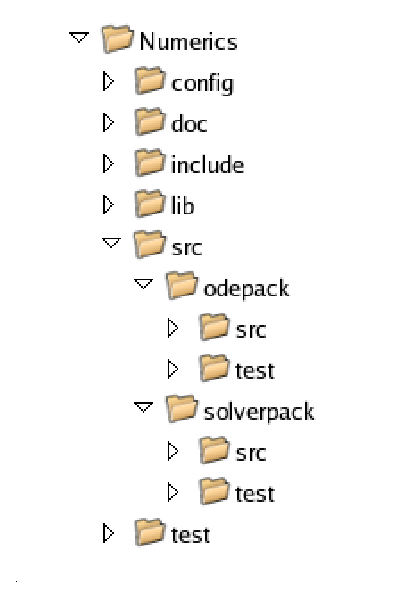
\includegraphics[scale=1.2, clip]{figure/NumericsDesign.eps}
	\caption{Tree view of the Numerics directories}
	\label{fig: Tree view of the Numerics directories}
	\end{center}
	\end{figure}
	
Each \textit{src} directory contains the source code of \ac{numerics}, especially \textit{src/odepack/src} and \textit{src/solverpack/src} which contain the code of \ac{ode} pack and MP solverpack.




\newpage
%---------------------------------------------------------------------------%
\chapter{Component description}
\label{Sec:ADD-ComponentDescription}
\section{Front-End Package}

	The class diagram \ref{fig: Class diagram for the front-end} shows the structure we will use for this package.
	
	\begin{figure}
	\begin{center}
	\includegraphics[bb=25 720 300 830, clip]{figure/class_frontend.ps}%35 540 560 830
	\caption{Class diagram for the front-end}
	\label{fig: Class diagram for the front-end}
	\end{center}
	\end{figure}
	


	\subsection{Component ``enter choice''}
		
		\begin{description}
	
		\item[Identifier~:]EnterChoice
		\item[Type~:]Method
		\item[Function-processing~:]Offer to read data or to run the simulation for the user. Transmits the result to the ``connect'' component.
		\item[Dependencies~:]-
		\item[Interfaces~:]Output : formalisation or simulation
		\item[Data~:]-

		\end{description}
	
	
  	\subsection{Component ``connect depending on choice''}
	
		\begin{description}
	
		\item[Identifier~:]Connect
		\item[Type~:]Method
		\item[Function-processing~:]Launch the read of the data or launch the simulation depending on the choice enter in the ``enterChoice'' component.
		\item[Dependencies~:]The component  ``enterChoice'' must be executed before this component is called.
		\item[Interfaces~:]Take as input the result of ``enterChoice''.
		\item[Data~:]-

		\end{description}

%  	\subsection{Component ``process manually input data''}
%	\begin{description}
%	\item[Identifier~:]ProcessManData
%	\item[Type~:]Module
%	\item[Function-processing~:]Process the data that are entered manually %using the interface. The data entered by the user (generally matrix
%	and function) are converted to a specified format in order to be %transmitted to the model formalisation package.
%	\item[Dependencies~:]The package  ``model formalisation'' must be %executed after this component is called.
%	\item[Interfaces~:]Take as input the data entered by the user.
%	\item[Data~:]-
%	\end{description}
	

	
\section{Model Formalisation Package}
	The class diagram \ref{fig: Class diagram for model formalisation} shows the structure we will use for this package.
	
	\begin{figure}
	\begin{center}
	\includegraphics[scale=0.85, bb=20 500 560 830, clip]{figure/class_formalisation.ps}
	\caption{Class diagram for model formalisation}
	\label{fig: Class diagram for model formalisation}
	\end{center}
	\end{figure}


	\subsection{Component ``fill dynamic system''}	
	
		\begin{description}
	
		\item[Identifier~:]FillDS
		\item[Type~:]Module
		\item[Function-processing~:]Fill the dynamic system part of the \ac{nsds}.
		\item[Dependencies~:]This component can be executed before, after or meanwhile the processing of the ``fill relations'' and the ``fill non smooth law'' component.
		\item[Interfaces~:]Take as input the data given by the Input/Output/Plug-in package. The output is the representation of the dynamic system.
		\item[Data~:]An inherited class of the DynamicSystem class.

		\end{description}
  	
	
	\subsection{Component ``fill relations''}
	
		\begin{description}
	
		\item[Identifier~:]FillRelations
		\item[Type~:]Module
		\item[Function-processing~:]Fill the relation part of the \ac{nsds}.
		\item[Dependencies~:]This component can be executed before, after or meanwhile the processing of the ``fill dynamic system'' and the ``fill non smooth law'' component.
		\item[Interfaces~:]Take as input the data given by the Input/Output/Plug-in package. The output is the representation of the relation.
		\item[Data~:]An inherited class of the Relations class.

		\end{description}
	
	
  	\subsection{Component ``fill non smooth laws''}
	
		\begin{description}
	
		\item[Identifier~:]FillNSLaw
		\item[Type~:]Module
		\item[Function-processing~:]Fill the non smooth laws part of the \ac{nsds}.
		\item[Dependencies~:]This component can be executed before, after or meanwhile the processing of the ``fill dynamic system'' and the ``fill relations'' component.
		\item[Interfaces~:]Take as input the data given by the Input/Output/Plug-in package. The output is the representation of the non smooth law.
		\item[Data~:]An inherited class of the NonSmoothLaw class.

		\end{description}

	
  	\subsection{Component ``update state''} \label{update_state}
	
		\begin{description}
	
		\item[Identifier~:]UpdateState
		\item[Type~:]Module
		\item[Function-processing~:]Update the state of the system when the model is formalised.
		\item[Dependencies~:]This component can be executed after the processing of the ``fill dynamic system'', ``fill relations'' and the ``fill non smooth law'' component, or after the ``computation'' execution (cf. section \ref{computations}).
		\item[Interfaces~:]Take as input data from the formalised model and save the system state with this data.
		\item[Data~:]System state

		\end{description}
	

\section{Numerical Strategy Package}

	The Class diagram \ref{fig: Class diagram for numerical strategy} shows the structure we will use for this package.
	
	\begin{figure}
	\begin{center}
	\includegraphics[bb=25 690 245 830, clip]{figure/class_numerical_strategy.ps}
	\caption{Class diagram for numerical strategy}
	\label{fig: Class diagram for numerical strategy}
	\end{center}
	\end{figure}
	
	


  	\subsection{Component ``increase time step''}
	
		\begin{description}
	
		\item[Identifier~:]IncreaseTimeStep
		\item[Type~:]Method
		\item[Function-processing~:]Give the signal for begin to simulate one time step
		\item[Dependencies~:]Its execution takes place before the ``predict interaction'' component execution
		\item[Interfaces~:]-
		\item[Data~:]-

		\end{description}
	
	
  	\subsection{Component ``predict interaction''}
	
		\begin{description}
	
		\item[Identifier~:]PredictInteraction
		\item[Type~:]Module
		\item[Function-processing~:]Predict the interaction between object.
		\item[Dependencies~:]This component can be executed only after ``increase time step''. It had to be executed before the ``verify constraint'' execution.
		\item[Interfaces~:]This component can use some functions defined in a specific plug-in. It uses the data stored in the system state to predict the interaction. 
		\item[Data~:]-

		\end{description}
	
  	\subsection{Component ``verify constraints''}
	
		\begin{description}
		
		\item[Identifier~:]VerifConstraints
		\item[Type~:]Module
		\item[Function-processing~:]Verify the constraint of the system (if 2 objects are not at the same place)
		\item[Dependencies~:]The component ``predict interaction'' must be executed before this component is called and ``make coherent'' 
		\item[Interfaces~:]This component can use some functions defined in a specific plug-in. It uses the data stored in the system state and the prediction of the interaction to verify the constraint.
		\item[Data~:]-

		\end{description}
	
  	\subsection{Component ``make coherent''}
	
		\begin{description}
	
		\item[Identifier~:]MakeCoherent
		\item[Type~:]Module
		\item[Function-processing~:]Make the system coherent if not
		\item[Dependencies~:]This component must be executed after ``verify constraint'' only if there is a constraint violation.
		\item[Interfaces~:]This component can use some functions defined in a specific plug-in. It uses the data stored in the system state and the data produced by the component ``verify the constraint'' to make the system coherent.
		\item[Data~:]-

	\end{description}
	
  	\subsection{Component ``computations''}\label{computations}
	
		\begin{description}
	
		\item[Identifier~:]Compute
		\item[Type~:]Module
		\item[Function-processing~:]Compute one time step using numerical libraries.
		\item[Dependencies~:]This component must be executed after ``verify constraint'' if there is non constraint violation and after ``make coherent'' in the other case.
		\item[Interfaces~:]This component can use some functions defined in a specific plug-in. It uses the data stored in the system state.
		\item[Data~:]-

		\end{description}
	
	\subsection{Component ``update state''} 
	cf. \ref{update_state}\\
	
	

\section{Input/Output/Plug-in Package}
	The Class diagram \ref{fig: Class diagram for specific plug-ins} shows the structure we will use for this package.
	
	\begin{figure}
	\begin{center}
	\includegraphics[bb=20 700 160 820, clip]{figure/class_specific_plugins.ps}
	\caption{Class diagram for specific plug-ins}
	\label{fig: Class diagram for specific plug-ins}
	\end{center}
	\end{figure}
	
	
  	\subsection{Component ``read \acs{xml} file''}
	
		\begin{description}
	
		\item[Identifier~:]ReadXML
		\item[Type~:]Module
		\item[Function-processing~:]Read the \ac{xml} file which describes the system state and the numerical strategy.
		\item[Dependencies~:]-
		\item[Interfaces~:]Take as input an \ac{xml} file and give in return the data and function describing the system.
		\item[Data~:]-

		\end{description}
	
  	\subsection{Component ``read and convert dedicated file''}
	
		\begin{description}
	
		\item[Identifier~:]ReadFile
		\item[Type~:]Module
		\item[Function-processing~:]Read and convert a dedicated file in order to have a description of the system state and the numerical strategy.
		\item[Dependencies~:]-
		\item[Interfaces~:]Take as input a specific file and give in return the data and function describing the system.
		\item[Data~:]-

		\end{description}
	
  	\subsection{Component ``bring out complete result''}
	
		\begin{description}
	
		\item[Identifier~:]CompletRes
		\item[Type~:]Module
		\item[Function-processing~:]Put the complete results in a \ac{xml} file
		\item[Dependencies~:]The computation of one time step must be finished.
		\item[Interfaces~:]Take as input the result of the component ``computation''.
		\item[Data~:]-

		\end{description}
	
  	\subsection{Component ``bring out partial result''}
	
		\begin{description}
	
		\item[Identifier~:]PartialResult
		\item[Type~:]Module
		\item[Function-processing~:]Put piece of results in a \ac{xml} file
		\item[Dependencies~:]The computation of one time step must be finished.
		\item[Interfaces~:]Take as input the result of the component ``computation''.
		\item[Data~:]-

		\end{description}



\newpage
%---------------------------------------------------------------------------%
\chapter{Architecture implementation : methods and softwares}
\label{Sec:ADD-ComponentImplementation}
\textit{This chapter precises methods and softwares who will be used to
implement the criticals points of the conceptual architecture described in the before chapters.}

\section{Plugin method}
A simple prototype named BPP has been developped to validate some functionnalities used by the plugins mechanism, like dynamic loading of libraries or
instantiation of objects encapsulated in a dynamic library. This prototype was also needed to verify portability of the libraries. \\
Another point tried with success was the possibility during the instanciation of a dynamical systems too indicate to the platform which computation method
(stored in a given library) has to be used. For example, for a lagrangien system, we can choose a particular function to compute the mass, etc. \\
The next step is to put together this prototype and XML functionnalities in a new prototype to validate our general idea of the functionning of our software.

\section{Fortran encapsulation}

In the \ac{srd}, Corba has been chosen to allow to re-use functions/libraries of other softwares (like \ac{lmgc90}). After a study, it appears that it is possible to make communication between C++ and Fortran languages (a Corba distribution exists), but it is not free. Consequently, to make a LMGC plugin, who may be implemented in the first version of the platform (see \ac{op}), a wrapper will be used.


%\section{C++ interpretor}
% description, pouqruoi on l'a choisi, portabilit�
%A way to use the computation's platform is to write a program in C++ and to run it without compiling it. In order to do that, a C++ interpretor is needed. \ac{cint} is the most famous C++ interpretor found
%on the web. We must insure that \ac{cint} answers our waitings.

\textbf{\ac{cint} specifications}
\begin{description}
	\item[Portability :] \ac{cint} works on number of operating systems. Linux, HP-UX, SunOS, Solaris,
	Windows-NT/95/98/Me, MacOS and with number of compilers, g++, HP-CC/aCC, Sun-CC/CC5, IBM-xlC,
	Compac-cxx, SGI-CC, Visual-C++, Borland-C++.
	\item[Features :] \ac{cint} covers about 95\% of ANSI C and 85\% of C++, supports the STL, allow to
	use embedded compiled C/C++ library code as shared objects.
	\item[Limitations :] \ac{cint} is not as powerfull as a C++ compiler. No "typedef" could be done, no
	overloading for operators, support of an old version of the STL.
\end{description}

A prototype as been created to test the abilities of \ac{cint}. The use of static libraries, templates, and
the STL in a prototype as shown that they can be used if libraries have simple headers (the use of
"makecint" is adviced), the templates are simple and if we use basic functions of the STL.



\section{\acs{xml} files management}

In order to manage the \ac{xml} files (data input/output), the LibXML2 library have been chosen.\\

LibXML2 is an \ac{xml} C parser and toolkit developed for the Gnome project (but usable outside of the Gnome platform). It is a free software available under MIT License. \\

\textbf{Why LibXML2?}

\begin{itemize}
\item Portability : LibXML2 is known to be very portable, the library should build and work without serious troubles on a variety of systems (Linux, Unix, Windows, MacOS, MacOS X, RISC Os,
 ...) ;
\item LibXML2 passes all 1800+ tests from the \ac{oasis} XML Tests Suite ;
\item Diversity : several APIs are implemented by LibXML2 like \ac{dom} or \ac{sax} ;

\end{itemize}

About the use and possibilities of LibXML2, it seems to be adapted and powerfull enought for our project : a prototype verifing, reading, and writing \ac{xml} files has been developed, and the
results are encouraging. The library has only a negative point : modules, methods and structures are summarily documented/specified.

\section{\acs{lmgc90} plugin}
\ac{lmgc90} is an existing software for mechanical computations. The aim of this plugin is to use theirs complex contact detection functions, so that only low level external methods are used. Simulation mechanisms don't change. It consists in communications between the \acs{kernel} and the \ac{lmgc90} plugin. 



\newpage
%---------------------------------------------------------------------------%
%\chapter{Logical validation and verification}
%\label{Sec:ADD-LogicalValidation}
%The logical validation and verification phase refers to the \ac{pti} document.


%\newpage
%---------------------------------------------------------------------------%


%\printglosstex(glo)[p]
\printglosstex(acr)[p]


\listoffigures
%\listoftables
%\cleardoublepage
%\bibliographystyle{plainnat}
%\bibliography{./Biblio/String,./Biblio/Cp.bib,./Biblio/Optim.bib,./Biblio/Contact.bib,./Biblio/NonSmooth.bib,./Biblio/Leger.bib,./Biblio/Petri.bib}
\cleardoublepage
\end{document} 
